\documentclass[12pt]{article}
\usepackage{graphicx} % For including graphics
\usepackage{hyperref} % For URLs and hyperlinks
\usepackage{amsmath} % For math symbols
\usepackage{enumitem} % For customized lists
\usepackage{geometry} % For page margins
\usepackage{xcolor} % For colored text
\usepackage{titlesec} % For title formatting
\usepackage{fancyhdr} % For headers
\usepackage{setspace} % For spacing
\usepackage{graphicx}
\usepackage{multirow}
\usepackage{adjustbox} % For scaling the table
\usepackage{array} % For defining column widths and centering
\usepackage{geometry} % For margin adjustments
\usepackage{booktabs} % For better looking tables
\usepackage{caption}
\usepackage{subcaption}
\usepackage{float}
\usepackage{rotating}      % For sideways tables
\usepackage{tabularx}      % For automatically adjusting column widths
\usepackage{enumitem}      % For controlling list spacing
\usepackage{placeins}  % For \FloatBarrier
\usepackage{caption}


% Page setup
\geometry{a4paper, margin=0.75in} % Adjust margins to allow more space
\setlength{\parindent}{0pt} % Remove indentation
\captionsetup{font=scriptsize}  % Change 'small' to any size: footnotesize, scriptsize, etc.




\renewcommand{\arraystretch}{1.2} % Adjusts the row height

% Title formatting with indentation for sections
% \titleformat{\section}{\bfseries\large\hspace*{1cm}}{\thesection.}{1em}{}
% \titleformat{\subsection}{\bfseries\hspace*{1cm}}{\thesubsection.}{1em}{}
% \titleformat{\subsubsection}{\bfseries\hspace*{2cm}}{\thesubsubsection.}{1em}{}

% Adjust paragraph indentation
\newenvironment{indentedsection}{
    \setlength{\parindent}{1cm} % Indent paragraphs
    \setlength{\leftskip}{1cm} % Indent entire section content
}{}

% Header setup
\pagestyle{fancy}
\fancyhf{}
\fancyhead[L]{Group No: C1}
\fancyhead[C]{ME 407 -- Fall 2024}
\fancyhead[R]{\thepage}

% Horizontal line
\renewcommand{\headrulewidth}{0.4pt}


% Begin Document
\begin{document}

% Main title and keyword section
\begin{center}
    \vspace{1em} % Add some space
    \textbf{\LARGE LITERATURE SURVEY}\\
    \vspace{1em} % Add some space
    \textbf{KEYWORD: Table Tennis, Ball Thrower, Ball Collector, Trajectory Control, Ping Pong Spin}
\end{center}

% Start of sections
\section{Introduction}

For this project of a table tennis pitching machine, a detailed literature survey that includes the research of commercial products available in the market, state of the art technologies and the patents is conducted. As the market for table tennis is wide and open for profit, there are already numerous of products and technologies on how to approach different aspects of the project.\\

For the commercial products, different table tennis ball pitching machines on the market are observed and analyzed to get an idea about their capabilities and shortcomings. It is necessary to choose which features to implement based on the demand on the market and the cost-effectiveness of the end product. \\

The state-of-the-art technologies are plenty for this project at hand, as there are multiple functions the machine must be able to perform. For aspects of launching, feeding itself from a reservoir, adjusting the speed and frequency etc., different kind of devices and mechanisms that can be used are investigated. \\

Lastly, the patents are an important part of the research, as intellectual properties must be respected, and should be taken into consideration so as to ensure the proceeding of the project does not arise any issues with copyright infringement.

\section{Commercial Products}

\begin{minipage}{0.6\textwidth}
    The table tennis table market is a vibrant sector in the sports and recreation sector, appealing to a variety of consumers from amateur players to professional athletes. The statistics in Figure \ref{fig:wholesales} below show the sales figures of table tennis equipment from manufacturers in the United States from 2007 to 2023. Last year, total sales of table tennis equipment in the United States reached approximately \$69 million in 2023. This was an increase of approximately 28\% compared to 2019. Therefore, it is naturally expected that the number of products and manufacturers in the market will increase. Also, according to research conducted by Business Research Insights, the global table tennis table market size was USD 485.3 million in 2022 and the market is expected to reach USD 598.11 million by 2032, growing at a CAGR of 2.1\% during the forecast period \cite{table_tennis_market_2032}.
\end{minipage}
\begin{minipage}{0.38\textwidth}
    \centering
    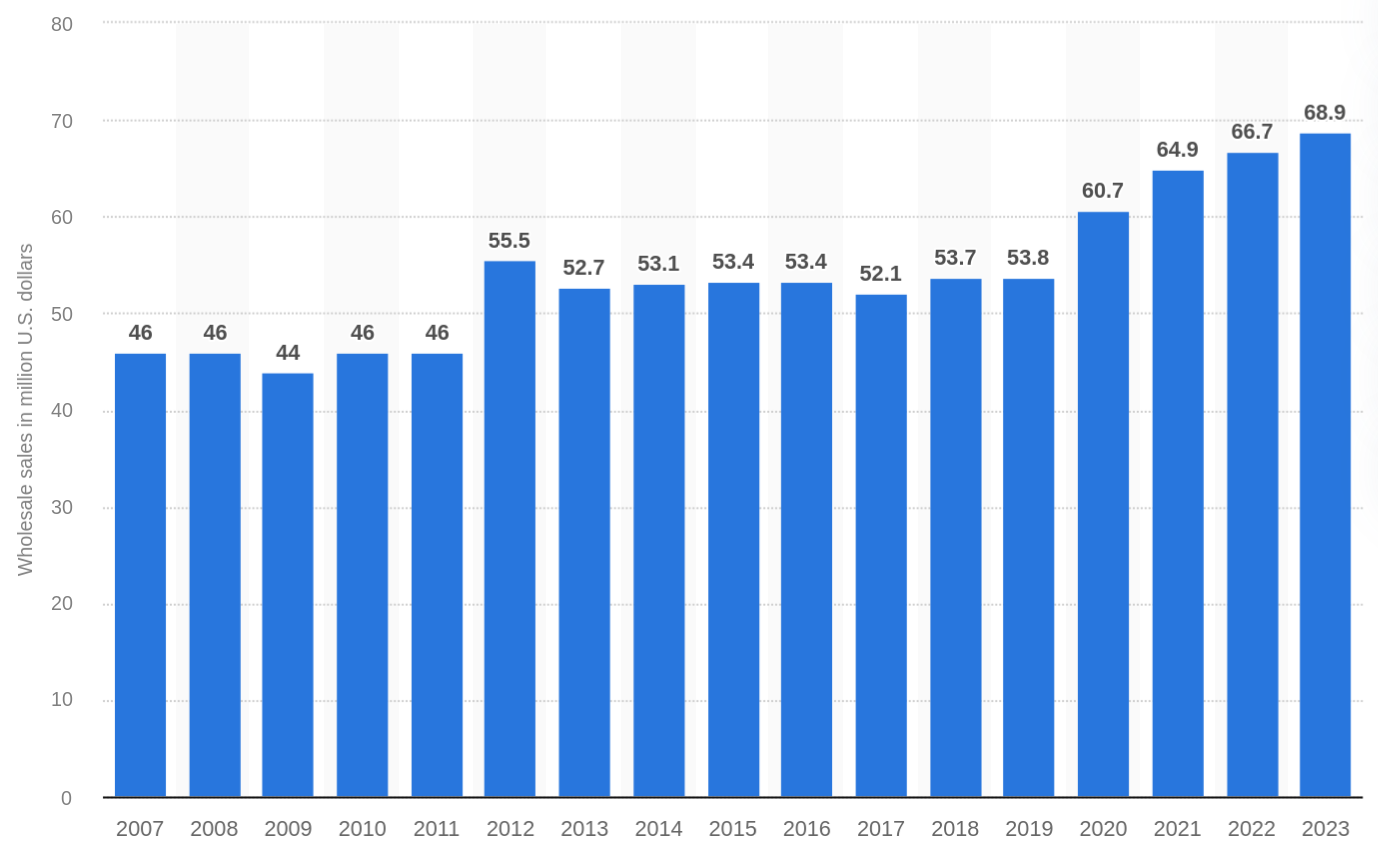
\includegraphics[width=\textwidth]{figures/wholesales.png}
    \captionof{figure}{Table tennis equipment wholesale sales in the U.S. from 2007 to 2023 \cite{statista2024}}
    \label{fig:wholesales}
\end{minipage}



After a careful research, various table tennis ball launcher models starting from \$100 and going up to \$2500 are found. One can see some common models, along with their comparisons in Table \ref{commercial} in Appendix. Of course, there are many differences in features among the devices in this wide price range. While affordable models can launch the ball without turning or by turning it only in one direction, advanced models can send the ball by turning it in 36 different ways. On the contrary, the dimensions of the ball chambers and the launch speeds are independent of the product prices. Almost all of the products, regardless of their prices, have launch speeds between 4 and 40 m/s. \\

In terms of usage, many products have wired or wireless control units. These units provide limited access with the buttons on them. It is seen that only in the highest segment products, the controller is in the form of a phone application. This feature should not be such a luxurious feature. This development may be a situation that is welcomed by many users. In addition, while doing this research it is seen that the ball turning mechanisms of various models are the same. Since the mechanism was the same, different rotations could not be obtained, but the number of rotations was increased by rotating the head section with smaller intervals. The research also shows that the products in this area could be further improved. \\

Several commercial products that serve the same purpose as the project requirements are reviewed. Most of the products are at an acceptable level at meeting the requirements but none of them fully meets the wanted requirements. The required max serving speed of 90 m/s couldn’t be achieved by any of the products. The max achieved speed is 40 m/s. One of the key requirements, the launch frequency, was almost achieved by most products, but fully achieved only by 4 products. These are the products of RoboPong and PowerPong. Considering the overall performance one can see that Robo Pong Super Pro and Robo Pong Pro Digital are the most suitable ones for the project requirements.

\section{State-of-the-Art on Related Technologies}

Recent developments in table tennis ball launchers, outlined in this section, focus on enhancing training efficiency and replicating real-game conditions. The literature survey identifies various studies exploring launch mechanisms and ball feeding systems that improve precision and control over key parameters. These advancements enable more precise training experiences, allowing players to better prepare for actual gameplay. This section states the findings from the literature on the latest innovations in table tennis ball launchers, highlighting their technical specifications and proposing directions for future research and development. 

\subsection{Launch Mechanisms}


Over the years, various pitching mechanisms have been developed, each with unique features designed to cater to different training needs. Among the most common are wheeled, pressurized, and hammered pitching machines  \cite{Lan2024}. Each mechanism offers different benefits, like precise control over ball speed, ability to give spin, adjust ball trajectory or realistic human-like trajectories. Understanding the differences in these machines’ mechanisms is crucial for selecting the right one to suit specific requirements of the project. 

\begin{indentedsection}

\subsubsection{Wheeled Pitching Machines}

Wheeled pitching machines utilize two or more spinning wheels to grip and propel the ball. The speed of the wheels can be adjusted independently, allowing for precise control over both speed and spin \cite{Dittrich2023}. By controlling the rotation speed of each wheel, users can simulate a variety of pitches making wheeled machines suitable for the project. Their ability to precisely control the trajectory, speed, and spin of the ball makes them a popular choice for both professional and amateur training environments (\cite{zxmoto2022}, \cite{amazon2024}, \cite{ipong2022} etc.). These mechanisms are also easier to manufacture compared to other pitching methods since only moving parts are the wheels that accelerate the ball \cite{Zhang2021}.

\subsubsection{Pressurized Pitching Machines}

Pressurized pitching machines function by using a compressed air system to propel the ball \cite{Wiley1994}. These machines are known for their ability to achieve very high ball speeds, which makes them ideal for practicing fastballs. However, they are limited in their ability to generate spin and control trajectory as effectively as wheeled machines. The air pressure can be adjusted to control the velocity of the pitch, but this type of machine is less versatile for training different types of pitches. Additionally, the need for a reliable air compressor makes these machines bulkier and less portable. 

\subsubsection{Hammered Pitching Machines}

Hammered pitching machines use a mechanical arm or hammer to strike and propel the ball forward. While this method simulates overarm throws or cricket bowling actions, it lacks the fine control over spin and speed that wheeled machines provide. These machines are often used for training where high consistency in delivery is necessary, but their lack of spin manipulation and limited speed control make them less effective for comprehensive training purposes. However, they offer a realistic simulation of  human-like throw, which may be advantageous in certain training scenarios. \\

\end{indentedsection}

Since wheeled mechanisms are superior in speed and trajectory control, the primary focus of the research was on these mechanisms and robots. There are various studies on different wheeled launch mechanisms in the literature. In the study of AIMY \cite{Dittrich2023}, they employed a three-wheel configuration to generate precise ball speeds, up to $15.4 m/s$, and spins up to $192.0 s^{-1}$, similar to professional human players.  Also, the study on table tennis robotic launchers \cite{Jamaludin2022} provides valuable insights into the development of launch mechanisms. The launch unit of table tennis robotic launchers predominantly employs one or two rotating wheels to propel the balls with variable speeds and spins. This system allows for precise control over ball velocities mTTTbot project utilizes two brushless motors connected to silicone wheels in the launch mechanism \cite{Tasci2023}. As noted by Jamaludin et al. \cite{Jamaludin2022}, the robot uses DC motors to generate spin and adjust the launching speed of the balls. By modifying the Pulse Width Modulation (PWM) values, the launch speed and distance can be controlled, which directly impacts the ball’s travel distance and spin during play. Apart from these, there are further studies in the literature not only specific to table tennis but also include diverse launch mechanisms which can also help us in our project. Distinct features in tennis ball machines, as described by Gao, contribute to the launch mechanisms \cite{Gao2019}. In Gao’s study, tennis balls are launched using two friction wheels with a 90 mm diameter and a 3 mm concave depth. These features improve grip and spin control, providing better ball speed and direction. The wheels are powered by 12V motors, allowing adjustable launch speeds and angles for versatile training. The concave design of the friction wheels enhances ball spin and control, making this design competitive with more expensive tennis ball machines.

\subsection{Ball Feeder}

The ball feeding system plays a critical role in maintaining a consistent and uninterrupted supply of balls to the launch mechanism, as demonstrated in several studies. The ball feeder in AIMY’s design offers precise control and reliability with its crank mechanism that converts the rotary motion of a servomotor into linear motion as shown in Fig.2, ensuring continuous feeding without clogging, which is ideal for long-duration training. However, the mechanical complexity may increase manufacturing and maintenance costs \cite{Dittrich2023}.Also, the table tennis robotic launcher described by Jamaludin et al. employs a hopper system that has high ball storage capacity, between 100 and 300 balls. The balls are delivered via a motorized conveyor belt or a rotating crank system, allowing for adjustable feed rates ranging from 25 to 80 balls per minute \cite{Jamaludin2022}. Apart from these, the mTTTbot project introduces a servo-driven feeding mechanism that continuously delivers balls through a helical channel, preventing interruptions in the training flow. As a drawback its reliance on continuous servo control could limit durability during extended use \cite{Tasci2023}. According to another study by Jamaludin et al., the ball feeder is driven by a motorized mechanism that supplies balls at a rate of 8 to 15 balls per minute under stationary conditions, although this rate decreases when the robot rotates to aim at different angles \cite{Jamaludin2023}. Expanding on the design concepts, Gao’s research on tennis ball machines includes a turntable mechanism that feeds balls into a guide rail with improved timing and frequency control. This system also prevents blockage between layers, enhancing the reliability of the feeding process during extended practice sessions \cite{Gao2019}. 

\vspace{0.5cm}\begin{figure}[H]
\centering
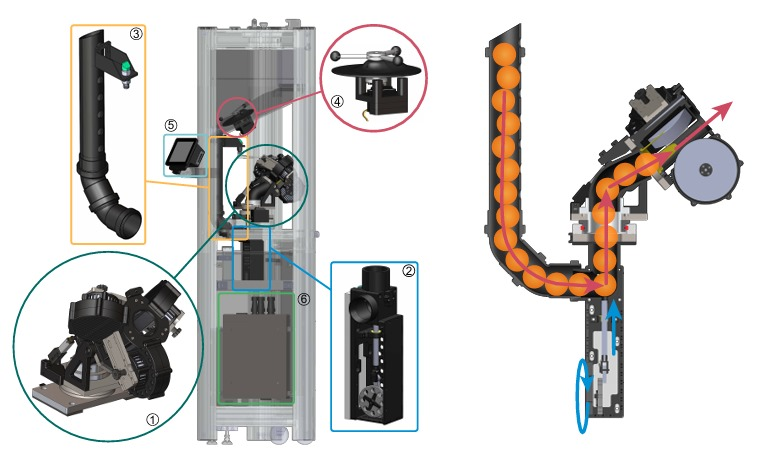
\includegraphics[width=0.45\textwidth,height=0.26\textwidth]{figures/fig2.jpg}
\caption{Sectional view of the ball feeding flow from the reservoir to launch unit in AIMY \cite{Dittrich2023}}
\end{figure}

\subsection{Reservoir}

The reservoir component plays an essential role in ensuring a continuous and uninterrupted supply of balls to the feeding system in robotic launchers. AIMY’s ball feeding system includes an optical sensor that monitors the ball supply and activates a stirrer to prevent clogging, ensuring a smooth flow of balls to the launch unit \cite{Dittrich2023}. In table tennis robotic launchers, as described by Jamaludin et al., the reservoir is designed to store a large number of balls (ranging from 100 to 300) and incorporates mechanisms to prevent clogging, ensuring consistent feeding to the launcher [2]. The mTTTbot system also features a ball reservoir that stores balls before feeding them into the launcher. A stirrer mechanism is integrated to prevent jams, further enhancing the operational reliability of the robot during training sessions [3]. In a study by Jamaludin et al., the ball reservoir is also equipped with a stirrer mechanism to prevent any clogging issues, like the AIMY robot [4]. In the case of tennis ball machines, Gao describes the use of a turntable reservoir with a two-layer design, which can hold up to 12 balls at once. While this design helps to avoid blockages between layers and ensures a smooth feeding process, its limited capacity may require more frequent reloading during prolonged practice sessions [5]. 

\subsection{Control Unit}

The control system is a pivotal component in the functionality of robotic ball launchers, allowing precise adjustments and remote management of the launch parameters. AIMY utilizes a Raspberry Pi as its control unit, enabling low-latency control (500 ms) through Ethernet or Wi-Fi, and providing an interface for integration with reinforcement learning (RL) environments via a Python API [1]. In a related study on table tennis robotic launchers, Jamaludin et al. describe the use of advanced user interfaces, which can be integrated with smartphone applications to control the system wirelessly via Bluetooth or Wi-Fi. These interfaces allow users to pre-program training routines and adjust variables such as spin, speed, and ball frequency for enhanced training realism [2]. The mTTTbot project also adopts an electronic control system that includes motor drivers, Bluetooth communication for remote control, and a microcontroller to manage all functions. The user-friendly mobile app interface facilitates easy adjustments of motor speeds, spin types, and shot angles, offering high flexibility for different training scenarios [3]. Jamaludin et al. further elaborates on an Arduino-based control system that manages the motors and movements, which is paired with a Bluetooth module for smartphone-based wireless control. This system leverages PWM control to fine-tune the speed and power supplied to the DC motors, enabling precise adjustments to the ball’s launch speed and travel distance [4]. Similarly, in the field of tennis ball machines, Gao’s research demonstrates the use of an STM32F407 microcontroller, which allows users to customize launch parameters such as speed, angle, and frequency, offering a highly responsive and versatile control experience [5].

\subsection{Actuators}

The selection and configuration of motors and actuators are crucial for controlling both the speed and spin of the balls in robotic launchers. AIMY utilizes high-performance brushless motors (T-MOTOR Antigravity MN5008 KV170) and servo motors to control the orientation and speed of the launch unit and ball feeding mechanism [1]. Similarly, in the table tennis robotic launcher described by Jamaludin et al., brushless motors are responsible for adjusting ball velocity and spin, while servo motors control the trajectory and launch angle to ensure precise delivery of balls during training sessions [2]. In the case of the mTTTbot, the launch unit operates with two brushless motors connected to silicone wheels, allowing for the generation of different types of spins, such as topspin, backspin, and sidespin, by adjusting the motor speeds [3]. Additionally, servo motors control the pitch, yaw, and roll axes of the launch head, providing precise adjustments for shot placement. According to Jamaludin et al., the robot uses DC motors to generate ball spin and adjust launch speed through Pulse Width Modulation (PWM) values, enabling fine-tuned control over ball travel distance [4]. Extending this approach to tennis ball machines, Gao’s research highlights the use of 12V DC motors that drive friction wheels with a concave design, enhancing ball grip and control over velocity and spin [5]. This combination of motors and actuators across different studies underlines their importance in achieving high precision and consistency in robotic launchers.



\vspace{1cm}In this state-of-the-art section, a comprehensive review of recent developments in table tennis ball launchers was conducted to inform the design of the project. In addition to that their advantages and disadvantages are discussed. Key mechanisms, including wheeled, pressurized, and hammered pitching systems, were analyzed to understand their respective strengths and limitations regarding speed, spin, and trajectory control. Ball feeding systems were explored to ensure continuous, jam-free ball supply for uninterrupted practice, while control units and actuator technologies were examined to enable precise adjustments and enhance the overall accuracy of ball delivery.  By studying these technologies, the most suitable components and designs for creating an efficient, adaptable, and realistic table tennis training system were identified. 

 
\section{Patents}
In this section, a review of existing patents related to table tennis ball launching machines is presented. This analysis aims to highlight innovative design approaches and technologies that were previously patented. By examining these patents, it is ensured that the design remains compliant with intellectual property laws while gaining insights into potential solutions that could inspire and guide the development of the project.
\subsection{Table Tennis Robot (US4765618A) \cite{Daley1988}}

\begin{minipage}{0.6\textwidth}  % Text takes 70% of the width
    This table tennis robot design aims to serve the ping-pong ball continuously at adjustable directions and methods, such as top-spin, back,and side-spins. This approach provides a more comfortable experience while practicing. The main idea here, which may be helpful, is that the balls are brought from bottom to top (from a lower level to a higher level), released to the serving mechanism and this procedure is continuously repeated. The serving mechanism consists of wheels to direct the balls. To accelerate the balls and satisfy the speed criteria, the design could be useful. However, on the other hand, depending on the elevation of the ball reservoir, the power-consumption may be excessive and design may be inconvenient. If the elevation is too high, the power needed to lift the balls could be quite high. To sum up, depending on the process and needs, this design could be beneficial and logical to implement.
\end{minipage}%
\hfill
\begin{minipage}{0.38\textwidth}  % Figure takes 28% of the width
    \centering
    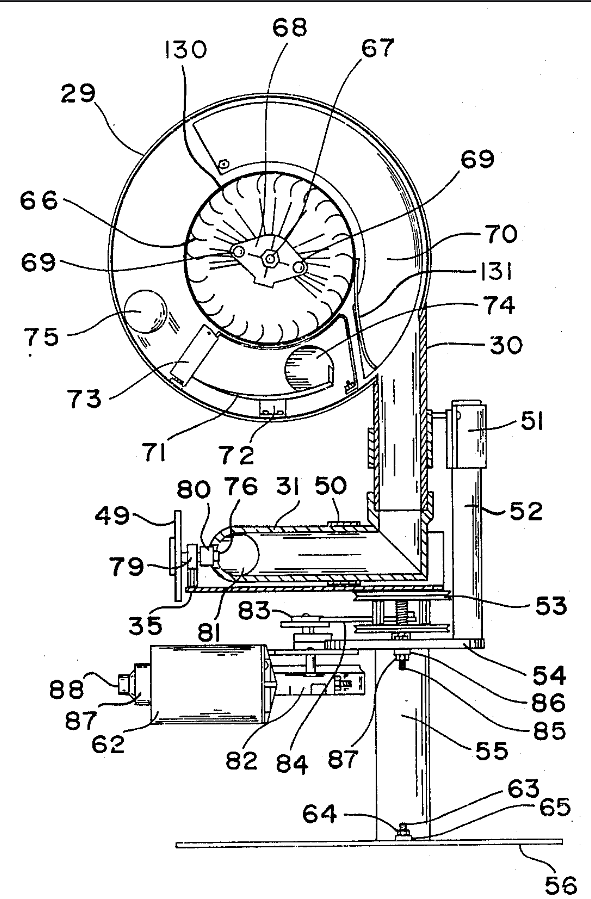
\includegraphics[width=0.47\textwidth]{figures/patent1-2.png}  % First image (48% width)
    \hfill
    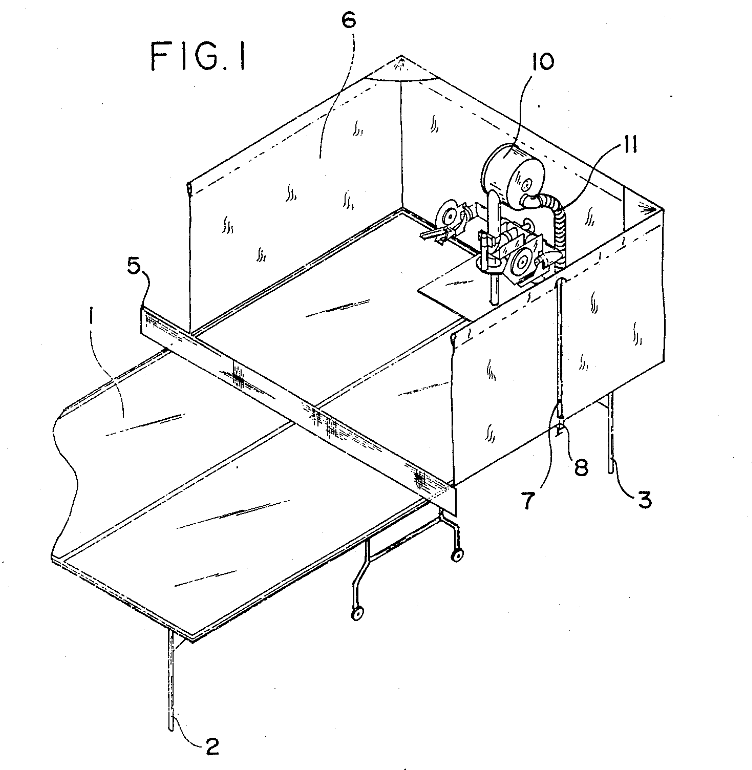
\includegraphics[width=0.48\textwidth,height=0.68\textwidth]{figures/patent1-1.png}  % Second image (48% width)
    \captionof{figure}{General System Description \cite{Daley1988}}  % Caption for both images
    \label{fig:pt1-2}
\end{minipage}


\subsection{Table Tennis Serving Machine (US6604517B1) \cite{Chao2003}}

\begin{minipage}{0.7\textwidth}  % Text takes 70% of the width
    This design is a much simpler and more incomplex example of an approach while constructing a table-tennis robot for those who would like to exercise and train by themselves. It basically consists of a gear system, ball reservoir segments capable of carrying 2 balls simultaneously, and a spring system to throw the ball. If the priority is simplicity, this design could be useful. Also, to achieve the desired speed, a stiff spring system could be useful. The main underlying reason that this design is patentable is that it replaces electronic components with mechanical components. Therefore, this design provides more simplicity. However, in terms of longevity, practicality, and ergonomics, this design is probably not the most usable one. The possible wear of the gear system may make the design unusable in a couple of years. In addition, the gear system could make the design heavy and difficult to carry.
\end{minipage}%
\hfill
\begin{minipage}{0.28\textwidth}  % Figure takes 28% of the width
    \centering
    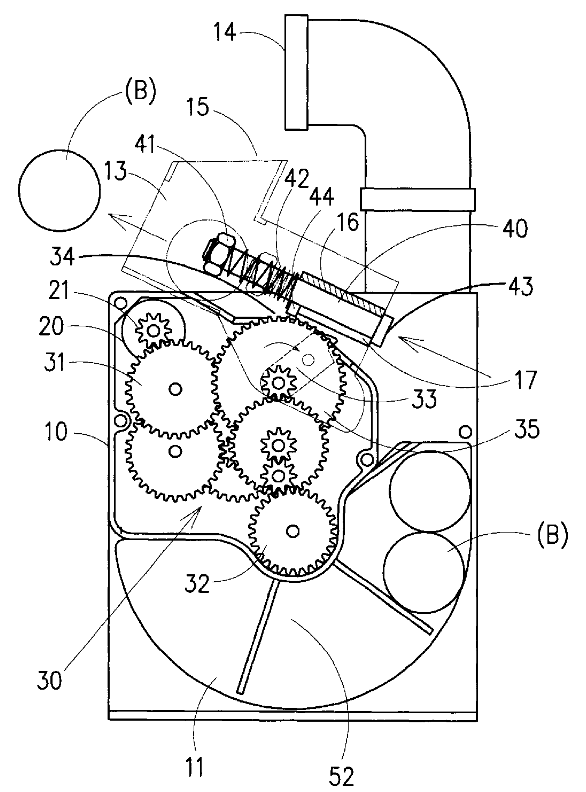
\includegraphics[width=\textwidth]{figures/patent2-1.png}
    \captionof{figure}{General schematic of serving machine \cite{Chao2003}}
    \label{fig:pt2-1}
\end{minipage}


\subsection{ Table Tennis Robot with Improved Serving Head Movement
 (EP3967376A1) \cite{Thoman2022}}

\begin{minipage}{0.7\textwidth}  % Text takes 70% of the width
     At that design, a ball feed collector can be seen. The main difference from the first design is that the internal pipe raises the balls to be able to throw them and this design raises the balls in a more effective way, since the ball collector reservoir is lower, which could be a key point for a good design. There are several servo motors and gears to adjust the thrower part. To exemplify, the thrower is able to move upwards and downwards, depending on the process desired, which enables the practice to have a more realistic experience. Also, the thrower part is adjustable so that the ball can be manipulated to make a top-spin, back-spin and side-spin type of throws. By the gear system, the angle of the thrower becomes adjustable. 
\end{minipage}%
\hfill
\begin{minipage}{0.28\textwidth}  % Figure takes 28% of the width
    \centering
    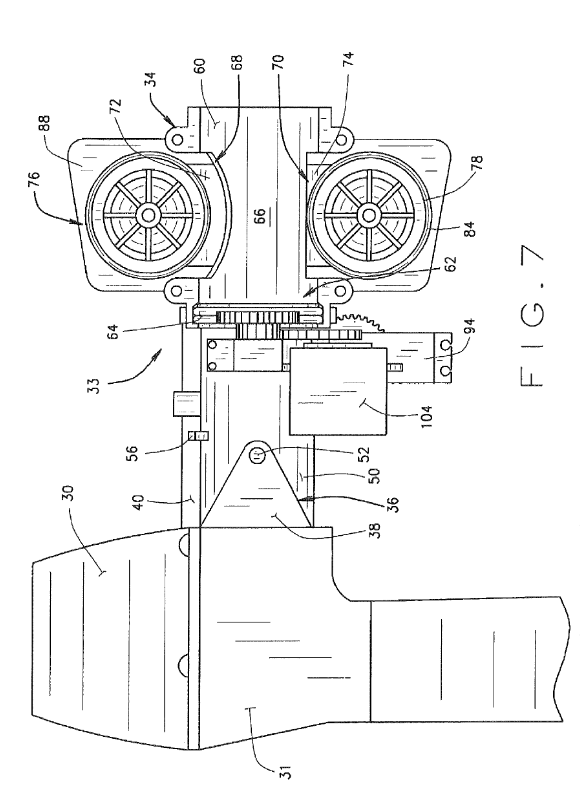
\includegraphics[width=0.9\textwidth]{figures/patent3-3.png}
    \captionof{figure}{Side view and detailed mechanism of table tennis robot \cite{Thoman2022}}
    \label{fig:pt3-1}
\end{minipage}

\begin{figure}[H]
    \centering
    \begin{subfigure}{0.4\textwidth}
        \centering
        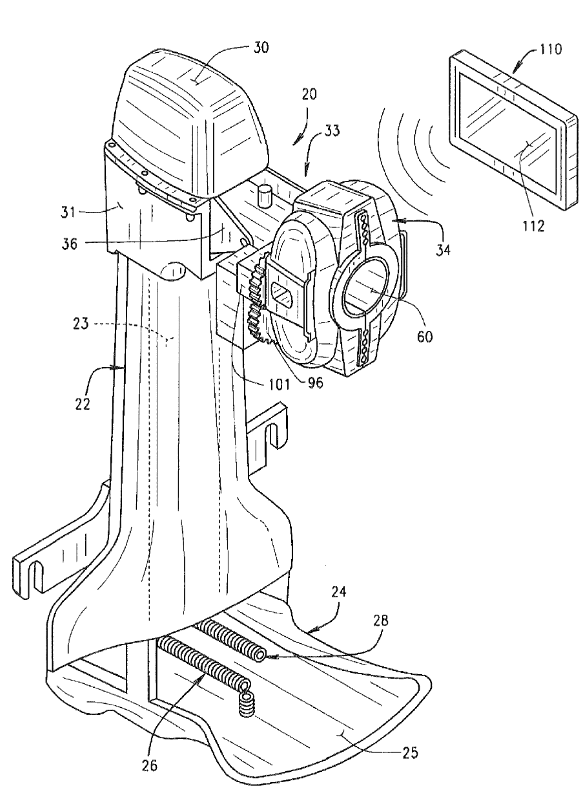
\includegraphics[width=0.45\textwidth]{figures/patent3-1.png}
        \caption{Orthogonal view}
    \end{subfigure}
    \hfill
    \begin{subfigure}{0.4\textwidth}
        \centering
        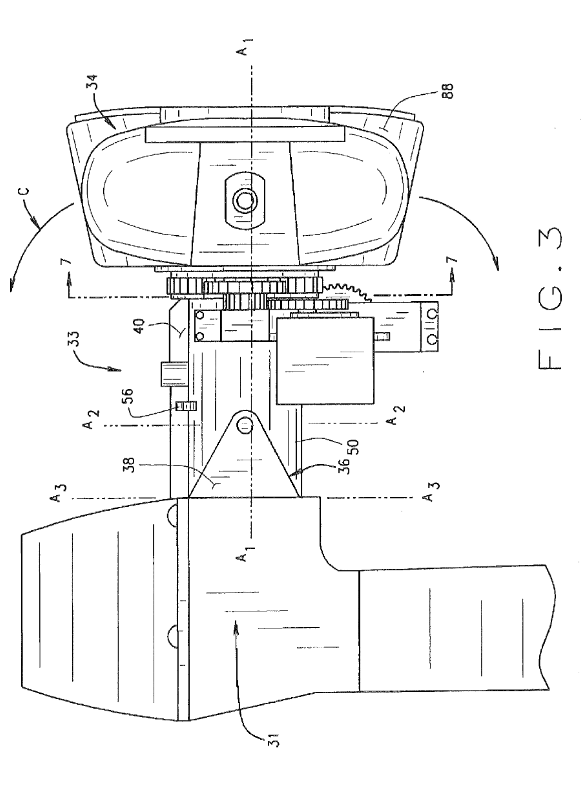
\includegraphics[width=.45\textwidth]{figures/patent3-2.png}
        \caption{General view}
    \end{subfigure}
    \caption{Orthogonal and general views of the table tennis robot \cite{Thoman2022}}
\label{fig:patetn3-2}
\end{figure}

\subsection{Programmable Ball Throwing Aparatus (US008287.4042B2) \cite{Romulo2012}}

\begin{minipage}{0.6\textwidth}  % Text takes 70% of the width
    In this device flight characteristics and field position parameters: spin, speed, ball trajectory are either programmed or manually selected by the user. The design is computer implemented and has built-in programs for different levels from beginner to expert. Also, it has specific modes for specific skill training like extreme backspin case. In addition, it allows users to program custom routines. The importance of this device for the project is that the planned product will also be adjustable for different flight parameters and trajectories. The underlying reason that this design is patentable comes from its programmability and freedom provided to the user.
\end{minipage}%
\hfill
\begin{minipage}{0.38\textwidth}  % Figure takes 28% of the width
    \centering
    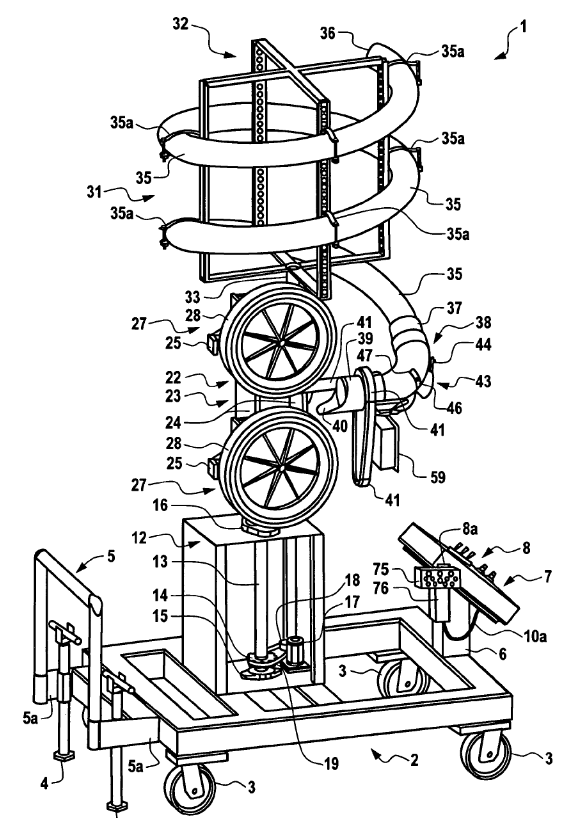
\includegraphics[width=0.48\textwidth]{figures/patent4-1.png}  % First image (48% width)
    \hfill
    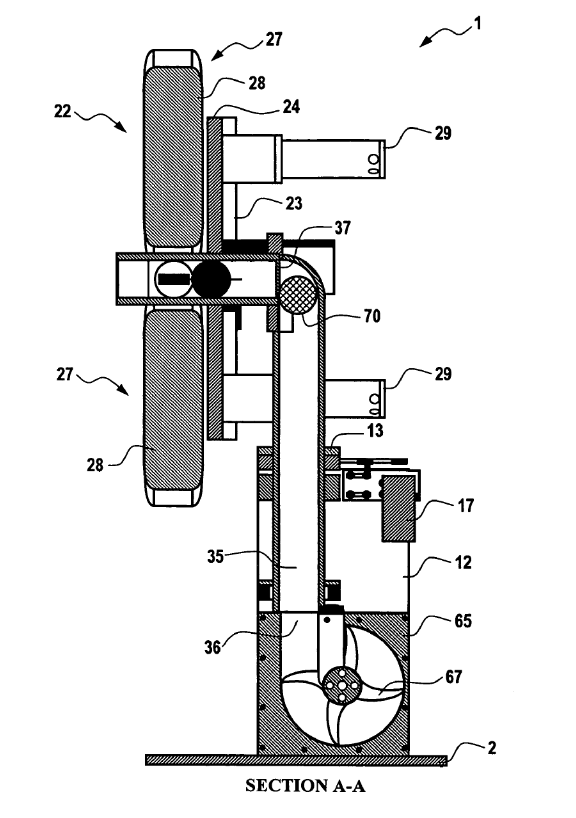
\includegraphics[width=0.48\textwidth]{figures/patent4-2.png}  % Second image (48% width)
    \captionof{figure}{General System Description \cite{Romulo2012}}  % Caption for both images
    \label{fig:patent4-1}
\end{minipage}

\subsection{Ball Throwing Device for Table Tennis (KR101992961B1) \cite{Kang2019}}

\begin{minipage}{0.6\textwidth}  % Text takes 70% of the width
    This patent describes a ball-throwing machine specifically designed for table tennis. The machine incorporates servomotors and various gears to control the ball's speed, spin, and direction. One key feature is its ability to continuously feed balls from a lower-level reservoir, reducing the machine's power consumption compared to designs with higher reservoirs. The ball thrower is adjustable for multiple spins (e.g., top-spin, back-spin), and the throwing mechanism is capable of providing angular adjustments for different ball trajectories. On the other hand, since the system can be constructed only once and it is not dispensable, this design may not meet the ergonomy criterion. 
\end{minipage}%
\hfill
\begin{minipage}{0.38\textwidth}  % Figure takes 28% of the width
    \centering
    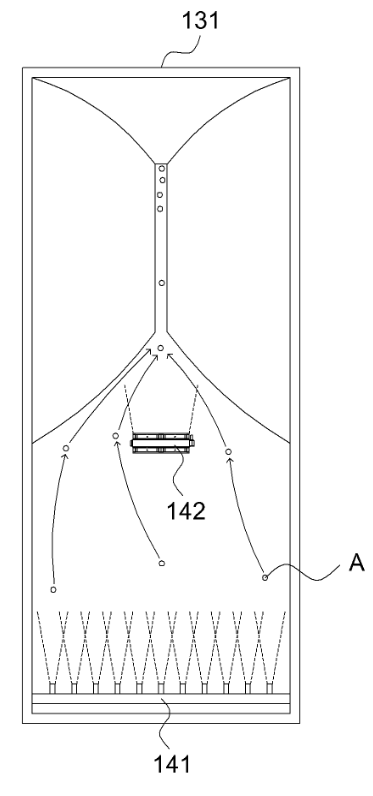
\includegraphics[width=0.48\textwidth,height=0.68\textwidth]{figures/patent5-1.png}  % First image (48% width)
    \hfill
    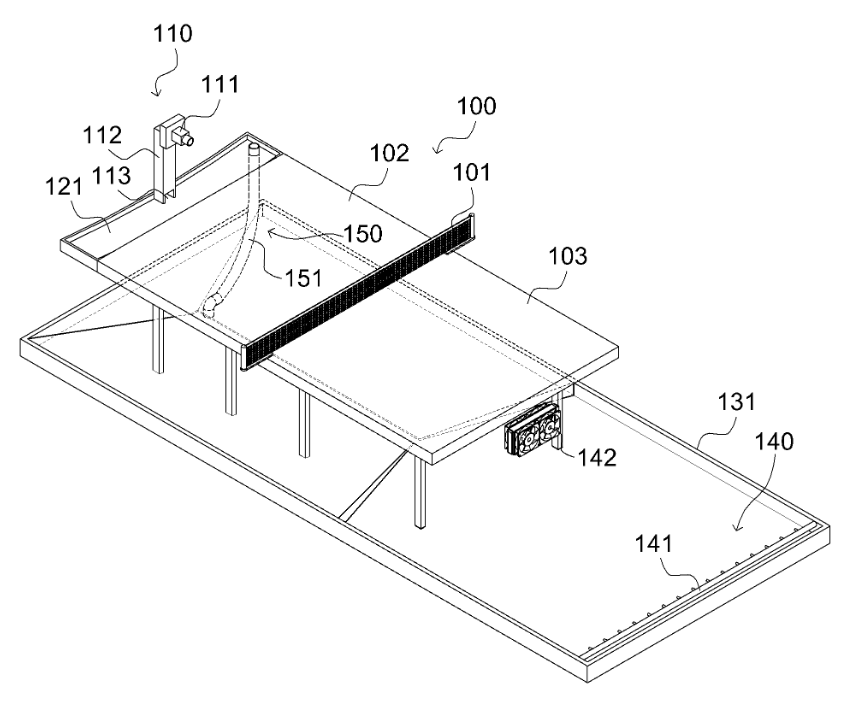
\includegraphics[width=0.48\textwidth,,height=0.78\textwidth]{figures/patent5-2.png}  % Second image (48% width)
    \captionof{figure}{Lower to Upper-Level Reservoir Feeding System \cite{Kang2019}}  % Caption for both images
    \label{fig:patent5-1}
\end{minipage}
\vspace{10pt}\\

The possible outcome of the research is, each of the designs has its advantages and disadvantages. The main idea is to be able to assess these designs wisely, get the ideas and inspiring points.


\section{Summary and Conclusion}
In this report, the results of a literature survey conducted spanning the commercial products in the market, state-of-the-art technologies and patents regarding the project at hand are presented. \\

A total of 10 commercial products are mentioned ranging from simple mechanical designs to highly advanced systems incorporating smart controls, whose different capabilities and aspects are studied to analyze their functions most useful to the project, and their shortcomings are discussed so as to how they could be improved upon, or be replaced with alternative solutions altogether. \\

State-of-the-art research made available many technologies and ideas that approach the technical problems encountered from different angles, and offer varying solutions to how the mechanisms operate. These different mechanisms are presented in detail to better understand their respective strengths and limitations regarding many technical aspects such as spin options, trajectory control, jam-free ball supply, enabling precise adjustments and accuracy. \\

A number of 5 patents are listed in this report, whose similarities and differences are discussed. Patents’ innovative approaches and methodologies to technical requirements including but not limited to power consumption, reserving and collecting the balls are mentioned to draw inspiration and compare the advantages and disadvantages of these designs. \\

In general, the information and ideas obtained from these research areas both gave rise to new inspiration and resulted in familiarizing with the many alternative solutions, while at the same time making apparent the need for a product to work upon the shortcomings and improve upon the strengths of the available designs to better simulate a real-life table tennis experience, thus enhancing the belief that this project will have a meaningful contribution to its field, and reinforcing the motivation to further work on it.

\newpage

\begin{sidewaystable}[h]
\centering
\scriptsize % Reduce font size
\begin{adjustbox}{width=\textwidth} % Scale the table to the text width
\begin{tabularx}{\textwidth}{|>{\centering\arraybackslash}X|>{\centering\arraybackslash}X|>{\centering\arraybackslash}X|>{\centering\arraybackslash}X|>{\centering\arraybackslash}X|>{\centering\arraybackslash}X|>{\centering\arraybackslash}X|>{\centering\arraybackslash}X|>{\centering\arraybackslash}X|>{\centering\arraybackslash}X|>{\centering\arraybackslash}X|}
\hline
\textbf{} & \textbf{PongBot Nova S Pro \cite{pongbotnova2024}} & \textbf{PowerPong Alpha \cite{powerpongalpha}} & \textbf{PowerPong Omega \cite{powerpongomega}} & \textbf{Huipang HP-07 \cite{huipanghp07}} & \textbf{Huipang S8-PRO \cite{huipangs8pro}} & \textbf{Huipang S1001 \cite{huipangs1001}} & \textbf{iPong V300 \cite{ipongv300}} & \textbf{Robo Pong Super Pro (3050) \cite{ipong2022}} & \textbf{Robo Pong Pro Digital (2055) \cite{robopong2055}} & \textbf{SIBOASI T899 \cite{siboasit899}} \\ \hline
\textbf{Price (USD)} & 350 & 1450 & 2195 & 256 & 763 & 172 & 140 & 2200 & 700 & 408 \\ \hline
\textbf{Length (cm)} & 46.5 & 24.1 & 24.1 & 39.4 & 88 & 41 & 28 & 28 & 28 & 165 \\ \hline
\textbf{Width (cm)} & 17.6 & 32.4 & 32.4 & 37.6 & 40 & 36 & 28 & 35.6 & 35.6 & 150 \\ \hline
\textbf{Height (cm)} & 34 & 78.7 & 78.7 & 35.8 & 41 & 32 & 48 & 83.8 & 83.8 & 78 \\ \hline
\textbf{Mass (kg)} & 4 & 10.89 & 10.89 & 4.42 & 7.5 & 4 & 1.25 & 8.15 & 10.9 & 5.4 \\ \hline
\textbf{Power (W)} & 24 & 24 & 24 & 36 & 50 & 36 & 50 & 50 & 50 & 60 \\ \hline
\textbf{Ball Frequency (balls per minute)} & 30-90 & 5-100 & 5-120 & 40-70 & 35-80 & 32-80 & up to 90 & 1-120 & 1-170 & 30-90 \\ \hline
\textbf{Ball Speed (m/s)} & 2-15 & 1-19 & 1-25 & 4-40 & 4-40 & 4-40 & 4-40 & 4-40 & 4-40 & 4-40 \\ \hline
\textbf{Capacity (balls)} & 200 & 100 & 100 & 120 & 200 & 120 & 100 & 120 & 120 & 80 \\ \hline
\textbf{No of spins} & 8 & 5 for topspin, 4 for backspin, 4 for right sidespin, 4 for left sidespin. & 7 for topspin, 5 for backspin, 6 for right sidespin, 6 for left sidespin. & 9 different spin options & 9 different spin options and no spin & 9 different spin options and no spin & 2 (Only Topspin and Backspin) & Topspin, Backspin, variety of side spins and no spin option & Topspin, Backspin, variety of side spins and no spin option & 4 \\ \hline
\textbf{Type of controller} & Mobile app + wireless remote controller & Control box and connects with a thin, light cable & No control box / Tablet or phone app can be used & Wired control box & Wireless remote & Wired control box & Wireless remote + digital panel & Mobile Application/Bluetooth & Digital Control box & Remote control \\ \hline
\textbf{Catch net to recycle balls} & - & + & + & - & + & - & - & + & + & + \\ \hline
\textbf{Material} & German BASF materials & Rubber + Metal & Rubber + Metal & Acrylonitrite butadiene styrene & Plastic + Metal & Plastic + Metal & Metal & Plastic + Metal & Plastic + Metal & Plastic + Metal \\ \hline
\textbf{Features} & \begin{itemize}[noitemsep, left=0pt, align=left]
    \tiny
    \item 20 to 30 up and down trajectory control
    \item Can be placed at 9 different positions on table
    \item Customizable spin, frequency, speed, oscillation, and trajectory settings
    \item Trajectory visualization on app
\end{itemize} & \begin{itemize}[noitemsep, left=0pt, align=left]
    \tiny
    \item 3 motors 120° degrees separated
    \item Allows many different shot types
    \item Has memory slots for shots
    \item Automatic Frequency Control
\end{itemize} & \begin{itemize}[noitemsep, left=0pt, align=left]
    \tiny
    \item 3 motors 120° degrees separated
    \item Allows many different shot types
    \item Unlimited memory for shots
    \item Individual Frequency Control
    \item Delay/Break time
\end{itemize} & \begin{itemize}[noitemsep, left=0pt, align=left]
    \tiny
    \item Rotating head for different spin directions
    \item 3 modes for trajectory angle
    \item Includes special Huipang balls reduce friction 
\end{itemize} & \begin{itemize}[noitemsep, left=0pt, align=left]
    \tiny
    \item Rotating head for different spin directions
    \item Adjustable head for trajectory angle
    \item Includes special Huipang balls reduce friction 
    \item Preset long/short ball, serve style practice
\end{itemize} & \begin{itemize}[noitemsep, left=0pt, align=left]
    \tiny
    \item Double heads for different types of serves
    \item Includes special Huipang balls reduce friction 
    \item Can serve two balls simultaneously
    \item 3 head modes for trajectory angle
\end{itemize} & \begin{itemize}[noitemsep, left=0pt, align=left]
    \tiny
    \item Includes tilt stand to change ball trajectory
    \item Can stand on its own
    \item Easily transportable
\end{itemize} & \begin{itemize}[noitemsep, left=0pt, align=left]
    \tiny
    \item Rotating head for different spin directions
    \item Different difficulty levels (Beginner to advanced)
    \item Advanced launching options
    \item Indicator lights that’s shows spin force and direction
\end{itemize} & \begin{itemize}[noitemsep, left=0pt, align=left]
    \tiny
    \item Rotating head for different spin directions
    \item Manually adjustable vertical tilt angle
    \item Different difficulty levels (Beginner to advanced)
\end{itemize} & \begin{itemize}[noitemsep, left=0pt, align=left]
    \tiny
    \item Rotating head for different spin directions
    \item Suitable for middle line ball, forehand ball, backhand ball trainings
\end{itemize}\\ \hline
\end{tabularx}
\end{adjustbox}
\caption{Comparison of Table Tennis Robots}
\label{commercial}
\end{sidewaystable}

% Prevent floats from passing this point
\FloatBarrier


% References section
\bibliographystyle{IEEEtran} % or any style you prefer
\bibliography{bibliography}

\end{document}
